\chapter{Generics}
\textbf{Generics} are an instance of \textit{Universal Polymorphism} with \textit{explicit parameters} (see Fig \ref{fig:polymorphism_classification}).

Consider arrays, which are \textit{homogeneous} collections of elements. An \lstinline|Array| type can work for any type \lstinline|T| because its implementation doesn't depend on any type-specific behavior: \ul{the \texttt{Array} implementation is uniform across all types}.

In fact they allow the same algorithm to be used with different types, which, however, must be explicitly declared.\\
In other languages, such as Haskell, \textit{type inference} allows the compiler to deduce the type of the parameters without the need for explicit declaration, implementing \textit{implicit} polymorphism.
\begin{paracol}{2}
   \begin{lstlisting}[caption={Java's explicit universal polymorphism}]
public <T> void printArray(T[] array) {
  for (T element : array) {
    System.out.println(element);
  }
}    
   \end{lstlisting}
 
   \switchcolumn

   \begin{lstlisting}[language=Haskell,caption={Haskell's implicit universal polymorphism}]
printList :: Show a => [a] -> IO ()
printList [] = return ()
printList (x:xs) = do
   print x
   printList xs         
   \end{lstlisting}
\end{paracol}

\section{Methods}
Methods can use the type parameters of the class
where they are defined, if any, but they can also introduce their own type parameters
\begin{lstlisting}
class MyList<T> {
   List <T> list = new ArrayList<T>();
   public T getFirst() {}
   public static <V> V getFirst(List<V> list) {}
\end{lstlisting}
Invocations of generic methods must instantiate all
type parameters, either explicitly or implicitly.
Some sort of \textit{type inference} is applied in case of implicit instantiation.

\subsection{Bounded Type Parameters}
\begin{lstlisting}
class NumList<E extends Number> {
      void m(E arg) {
            arg.intValue();   // OK, since...
            // Number and its subtypes support intValue()
         }
   }
\end{lstlisting}

Type parameters can also be \textbf{bounded} as in the above example,
allowing methods (and fields) defined in the \textbf{bound} to be invoked on objects of the type parameter \lstinline|T|.\\
There may be various kinds of type bounds:
\begin{lstlisting}
<TypeVar extends SuperType>
   // UPPER bound; SuperType and any of its subtype are ok.
<TypeVar extends ClassA & InterfaceB & InterfaceC & ...>
   // MULTIPLE UPPER bounds
<TypeVar super SubType>
   // LOWER bound; SubType and any of its supertype are ok
\end{lstlisting}

Unlike C++ where \textit{overloading} is resolved and can \textbf{fail} after
instantiating a template, in Java \textbf{type checking} ensures that
overloading will succeed.

\section{Inheritance and Arrays}
\subsection{SubTyping (Inheritance)}
There are two major issues which came up along with generics.
The first one regards \textbf{inheritance}; 
consider the following example:
\begin{center}
   Since \lstinline|Integer| is a \textit{subtype} of \lstinline|Number|,\\
   is \lstinline|List<Integer>| \textit{subtype} of \lstinline|List<Number>|?\nl

   {\color{red}\textbf{\textit{NO!}}}
\end{center}
In a formal way, \ul{\textit{subtyping is invariant} for Generic classes}.
Informally, given \lstinline|A,B| concrete types, \lstinline|MyClass<A>| has no relationship to \lstinline|MyClass<B>|,
even if \lstinline|A,B| have one.\\
On the other hand if \lstinline|A extends B| and are \textit{generic} classes, 
then \lstinline|A<C> extends B<C>| for any type \lstinline|C|.
For example, \lstinline|ArrayList<Integer> extends List<Integer>|.
\note{
   Note that the common parent of \lstinline|MyClass<B>| and \lstinline|MyClass<A>| is \lstinline|MyClass<?>|.
   This misty wildcard \lstinline|?| will be discussed later.
}
\nl

\subsection{Covariance - ``More specific output''}
Let's now discuss \textbf{covariance} and \textbf{contravariance}, with the aid of a few examples.

\begin{lstlisting}
List<Integer> lisInt = new ...;
List<Number> lisNum = new ...;
//lisNum = lisInt; // COMPILER ERROR - Reassign pointer
lisNum.add(new Number(...)); // NOT ALLOWED
//listInt = lisNum; // COMPILER ERROR - Reassign pointer
Integer n = lisInt.get(0); // NOT ALLOWED
\end{lstlisting}

\lstinline|List<Integer>| is neither a subtype or a supertype of \lstinline|List<Number>|,
thus the above operations aren't allowed.
However there are \textit{read-only} and \textit{write-only} situations where they may be allowed.

\begin{lstlisting}
RO_List<Integer> lisInt = new ...;
RO_List<Number> lisNum = new ...;
//lisNum = lisInt; // COMPILER ERROR
Number n = lisNum.get(0); // OK
\end{lstlisting}
Covariance refers to the ability to substitute a subtype where a supertype is expected. In simpler terms, it means that if you have a class \lstinline|RoList<Number>|, you should be able to use \lstinline|RoList<Integer>| wherever \lstinline|RoList<Number>| is expected, because \lstinline|Integer| is a subtype of \lstinline|Number|.\\
\ul{This is in Java allowed only for \textit{read-only} operations}.
It is ok to \textit{read} a \textbf{supertype} starting from a \textbf{subtype}.
\begin{center}
   \textit{\textbf{covariance} is safe if the type is \textbf{read-only}}
\end{center}

In Java everything is invariant by default -except for \lstinline|arrays[]|, which are covariant-, but it is possible to use \textit{wildcards} to allow covariance and contravariance.

Let's provide a different example to understand the concept of covariance:
you can assign to a \textit{covariant \texttt{Fruit} list} a list of \texttt{Apples}, because \texttt{Apples} are a subtype of \texttt{Fruit} and you can legally read from a \texttt{Fruit} list an \texttt{Apple}, since it is a \texttt{Fruit}.
However, you cannot write any subtype of \texttt{Fruit} in a covariant \texttt{Fruit} list, because such thing would allow you to add a \texttt{Banana} in a list of \texttt{Apples}, which we don't want. So\dots \textbf{read-only}.

This implicitly happens with \textit{wildcards} in Java, while in other languages such as C\# and Scala, when a class is declared as \textit{covariant}, limitations are applied to the class itself.

\subsection{Contravariance - ``More general input''}
\begin{lstlisting}
WO_List<Integer> lisInt = new ...;
WO_List<Number> lisNum = new ...;
//lisInt = lisNum; // COMPILER ERROR
lisInt.add(new Integer(...)); // OK
\end{lstlisting}
Contravariance allows a supertype to be substituted where a subtype is expected. In simpler terms, it means that if you have a class \lstinline|WoList<Integer>|, you should be able to use \lstinline|WoList<Number>| wherever \lstinline|WoList<Integer>| is expected, because \lstinline|Number| is a supertype of \lstinline|Integer|.\\
\ul{This is in Java allowed only for \textit{write-only} operations}.
It is ok to \textit{write} a \textbf{subtype} in the place of from a \textbf{supertype}.
\begin{center}
   \textit{\textbf{contravariance} is safe if the type is \textbf{write-only}}
\end{center}

\framedt{Copilot example}{

   So, let's go back to fruit. Imagine you have a contravariant function \lstinline|FruitJuicer.juice(List<Fruit> v)| that accepts a list of \texttt{Fruit} and processes it. This function can also accept a list of \texttt{Apples}, because \texttt{Apples} are a subtype of \texttt{Fruit}. 

   Hence, you can use the \texttt{Fruit} processor \lstinline|FruitJuicer.juice()| in place of a \textit{contravariant \texttt{Apple} processor}, because it can process any fruit! Including apples\smiley.

   What you can't do, is reading, because you can't read an \texttt{Apple} from a \texttt{Fruit} list, since it could be a \texttt{Banana}.

   
   In summary, contravariance allows you to use a more generic type (like \texttt{Fruit}) where a more specific type (like \texttt{Apple}) is expected, if the only operation is writing (processing).

   Note however, that in this scenario, the class \lstinline|FruitJuicer| would be a ``subtype'' of \lstinline|AppleJuicer|, because it can \textit{substitute} it.
}

\subsection{Covariance vs Contravariance}

\begin{paracol}{2}
   \begin{figure}[htbp]
      \centering
      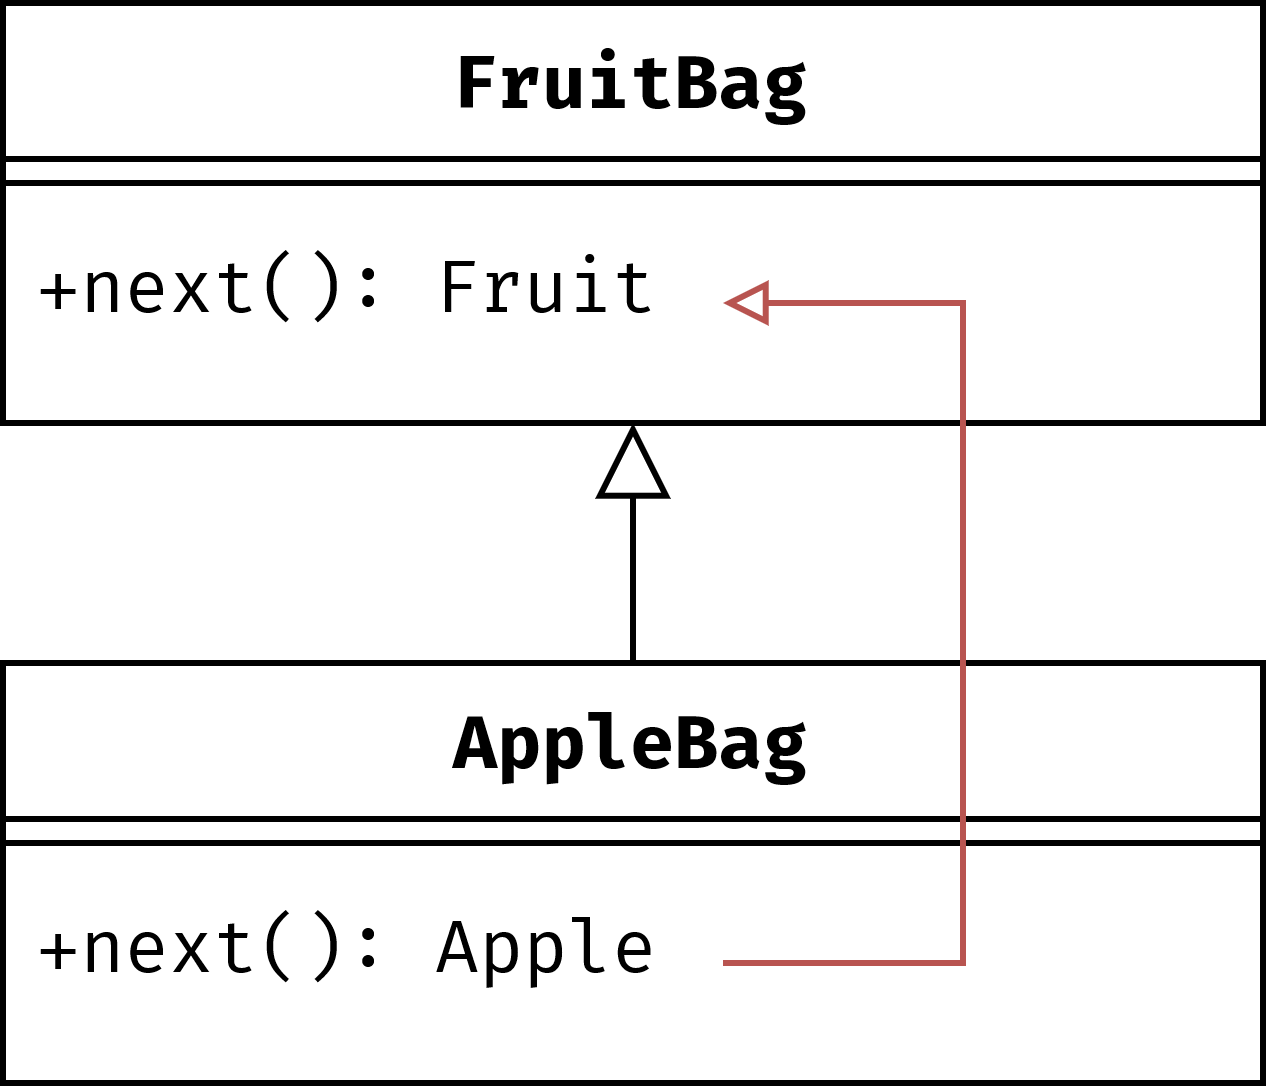
\includegraphics{images/variance1.png}
      \caption{Covariant Fruit Bag}
      \label{fig:variance1}
   \end{figure}
   \begin{lstlisting}
   If A:B then I<A>:I<B>
   \end{lstlisting}
   \coolquote{
      ``Be conservative in what you do''
   }{}

   Covariance in \textbf{output} types.
   
   \switchcolumn

   \begin{figure}[htbp]
      \centering
      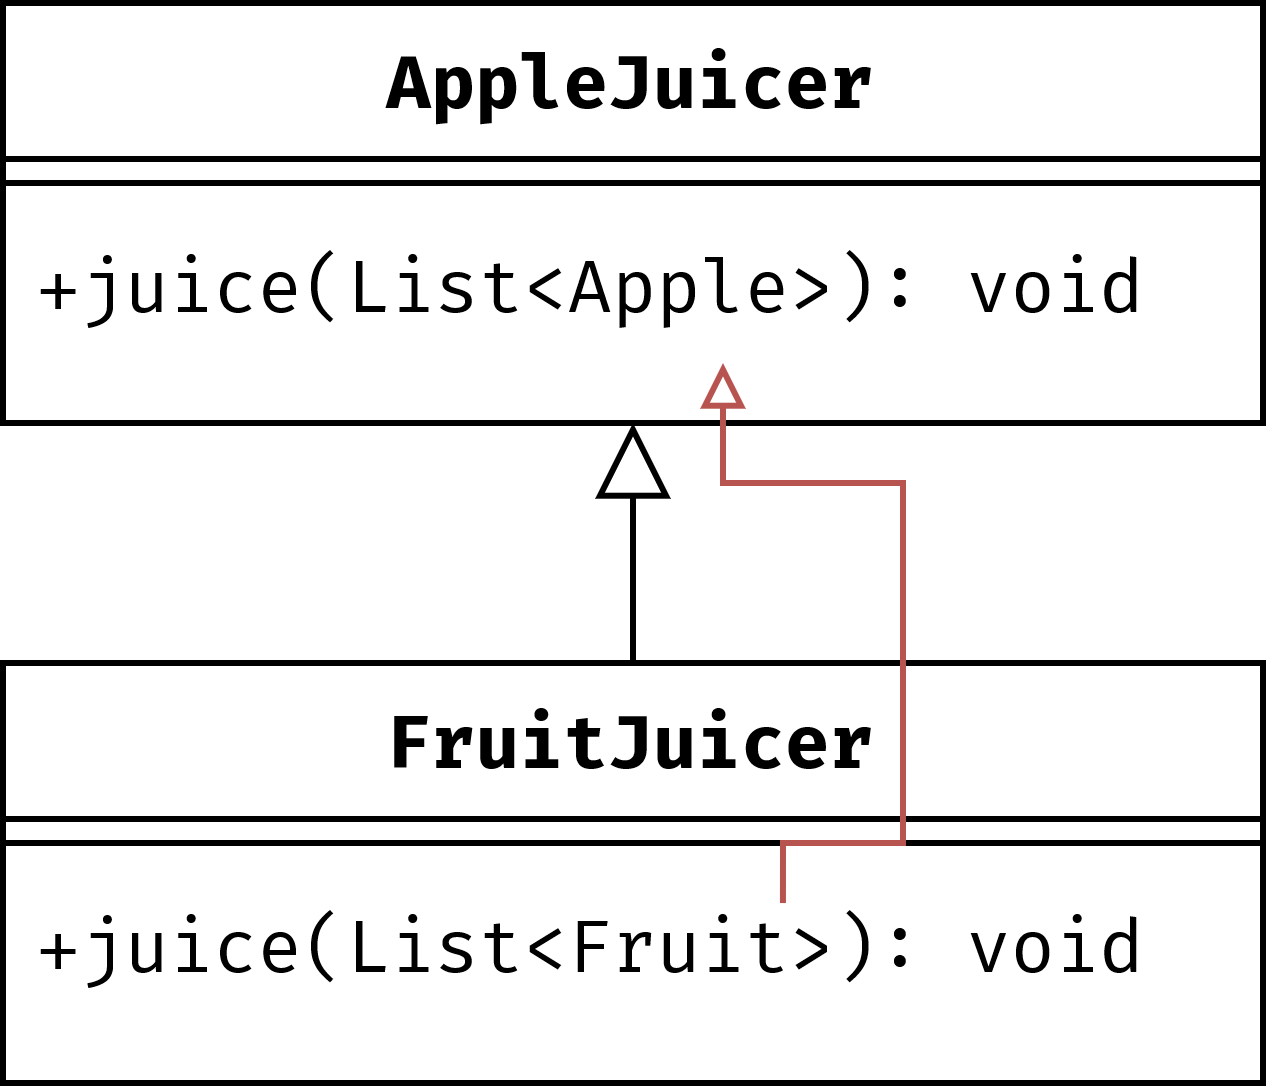
\includegraphics{images/variance2.png}
      \caption{Contravariant Apple Juicer}
      \label{fig:variance2}
   \end{figure}
   \begin{lstlisting}
   If A:B then I<B>:I<A>
   \end{lstlisting}
   \coolquote{
      ``Be liberal in what you accept from others''
   }{}

   Contravariance in \textbf{input} types.

\end{paracol}

\subsection{Wildcards}
\textbf{Wildcards} are strongly related to the topic of \textit{covariance} and \textit{contravariance}.\\
As briefly mentioned before, wildcards are the only relationship between generic classes.

To use \textit{wildcards}, the \textbf{PECS} principle is applied:
\textit{\textbf{P}roducer \textbf{E}xtends, \textbf{C}onsumer \textbf{S}uper}.
\begin{itemize}
   \item \lstinline|? extends T| to \textbf{get} values from a \textit{Producer}: \textbf{covariance} allowed
   \item \lstinline|? super T| to \textbf{insert} values into a \textit{Consumer}: \textbf{contravariance} allowed
   \item Never use \lstinline|?| when both insertion and retrieving is needed, \lstinline|T| is sufficient and way more appropriate.
\end{itemize}



Wildcards improve type-safety, allowing a program to fail at \textit{compile-time} instead of \textit{runtime}.
\begin{lstlisting}
List<Apple> apples = new ArrayList<Apple>();
List<? extends Fruit> fruits = apples;
fruits.add(new Strawberry()); // COMPILING FAILS :)
\end{lstlisting}

% \section*{17 - Ottobre}
\subsubsection*{Other languages}
In the case of \textbf{C\#}, generic classes can be marked with the keyword \lstinline|out| (\textit{covariant}) or \lstinline|in| (\textit{contravariant}),
otherwise the class is invariant.
In \textbf{Scala} the same happens,
but with the \lstinline|+| or \lstinline|-| operators.\nl

\subsection{Arrays}
Let's now discuss \textbf{arrays}.\\
Let \lstinline|A extends B|, then \lstinline|A[] extends B[]| even if instead \lstinline|Array<A>| is not related to \lstinline|Array<B>|.
\begin{center}
   Thus, \textit{arrays in Java are \textbf{covariant}.}
\end{center}

However there is a counterpart, since this allows rule-breaking assignments
which are allowed by the compiler but which lead to a runtime \lstinline|ArrayStoreException|.
This happens because the dynamic type of an array is checked at runtime.
Knowing this, for each array update, a runtime check is performed by the JVM which throws the exception if needed.
\begin{lstlisting}
Apple[] apples = new Apple[1];
Fruit[] fruits = apples;      // Ok, covariance
fruits[0] = new Strawberry(); // Compiles!
// Throws ArrayStoreException at runtime
\end{lstlisting}

After compilation Generic are all \textbf{type-erasured} to \lstinline|Object| or to their first \textit{bound}, if present.
This choice has been made mainly for compatibility with legacy code, leading all instances of the same generic type to have the same type at runtime; 
i.e.
\begin{lstlisting}
   List<String> lst1 = new ArrayList<String>();
   List<Integer> lst2 = new ArrayList<Integer>();
   assert(lst1.getClass() == lst2.getClass())   // true!
\end{lstlisting}

\subsubsection{Generic Arrays}
What about \textit{arrays of generics}?
Such arrays in Java are \textbf{not allowed},
because every array update needs a runtime check which is impossible to perform on generics,
since at runtime generics are all of the same type due to \textit{type-erasure}.


\section{Generics Limitations}
\begin{itemize}
   \item Cannot instantiate Generics with primitive types:
   \begin{lstlisting}
      ArrayList<int> a = ...                       // compile error
   \end{lstlisting}
   \item Cannot create instances of type parameters
   \item Cannot declare static fields whose types are type parameters
   \begin{lstlisting}
      public class C<T>{ public static T local; ...}
   \end{lstlisting}
   \note{Because static fields are represented in the \textbf{unique} representation of the class in the dedicated static memory area of the JVM for classes}
   \item Cannot use casts or instanceof with parameterized types
   \begin{lstlisting}
      mylist instanceof ArrayList<Integer>         // fails
      mylist instanceof ArrayList<?>               // OK
   \end{lstlisting}
   \item Cannot create arrays of parameterized types
   \item Cannot create, catch, or throw objects of parameterized types
   \item Cannot overload a method where the formal parameter types of each overload erase to the same raw type.
   \begin{lstlisting}
      public class Example {                       // does not compile
         public void print(Set<String> strSet) { }
         public void print(Set<Integer> intSet) { } }
   \end{lstlisting}
\end{itemize}

